
% NEW SLIDES: Statistical Methods Comparison

\begin{frame}
    \frametitle{Statistical Analysis Methods in Field Trials}
    
    \begin{columns}[T]
        \begin{column}{0.5\textwidth}
            \begin{block}{Traditional Approach}
                \textbf{Randomized Complete Block Design (RCBD)}
                \begin{itemize}
                    \item Assumes blocks capture all spatial variation
                    \item Fixed block effects
                    \item Cannot model continuous spatial patterns
                    \item Residual spatial structure ignored
                \end{itemize}
            \end{block}
        \end{column}
        
        \begin{column}{0.5\textwidth}
            \begin{block}{Geostatistical Approach}
                \textbf{Spatial Analysis Methods}
                \begin{itemize}
                    \item Model spatial correlation explicitly
                    \item Continuous spatial trends
                    \item Better residual structure
                    \item Improved precision
                \end{itemize}
            \end{block}
        \end{column}
    \end{columns}
    
    \vspace{1em}
    
    \begin{alertblock}{Research Question}
        Can geostatistical methods provide better estimates when environmental variation is not perfectly captured by experimental blocks?
    \end{alertblock}
\end{frame}

\begin{frame}
    \frametitle{Simulated Trial Design}
    
    \begin{columns}[T]
        \begin{column}{0.6\textwidth}
            \begin{block}{Experimental Setup}
                \begin{itemize}
                    \item 3 treatments × 3 blocks (9 plots)
                    \item 15m × 10m plots with 17 measurement points each
                    \item \textbf{Spatial gradient:} -1.5 to +1.5 t/ha across field
                    \item \textbf{Treatment effects:} Control (0), Test (+2), Reference (+1) t/ha
                \end{itemize}
            \end{block}
            
            \begin{block}{Key Issue}
                Blocks are \textcolor{red}{not perfectly aligned} with environmental gradient, creating spatial confounding
            \end{block}
        \end{column}
        
        \begin{column}{0.4\textwidth}
            \begin{table}[h]
                \centering
                \scriptsize
                \begin{tabular}{|c|c|c|}
                    \hline
                    \rowcolor{lightblue} \textbf{Block 1} & \textbf{Block 2} & \textbf{Block 3} \\
                    \hline
                    Test & Control & Reference \\
                    Reference & Test & Control \\
                    Control & Reference & Test \\
                    \hline
                \end{tabular}
                \caption{Randomization Layout}
            \end{table}
            
            \vspace{0.5em}
            
            \begin{block}{Spatial Pattern}
                \small
                \textbf{Environmental gradient:}\\
                West → East: 10.3 → 14.2 t/ha
            \end{block}
        \end{column}
    \end{columns}
\end{frame}

\begin{frame}
    \frametitle{RCBD Analysis Results}
    
    \begin{columns}[T]
        \begin{column}{0.5\textwidth}
            \begin{block}{Model Specification}
                $$Y_{ij} = \mu + \tau_i + \beta_j + \varepsilon_{ij}$$
                \begin{itemize}
                    \item $\mu$: overall mean
                    \item $\tau_i$: treatment effect
                    \item $\beta_j$: block effect
                    \item $\varepsilon_{ij}$: random error
                \end{itemize}
            \end{block}
            
            \begin{block}{Treatment Estimates}
                \scriptsize
                \begin{tabular}{lcc}
                    \hline
                    Treatment & Effect & SE \\
                    \hline
                    Control & 0.00 & -- \\
                    Reference & +2.03 & 0.089 \\
                    Test & +2.41 & 0.089 \\
                    \hline
                \end{tabular}
            \end{block}
        \end{column}
        
        \begin{column}{0.5\textwidth}
            \begin{block}{ANOVA Table}
                \scriptsize
                \begin{tabular}{lcccc}
                    \hline
                    Source & DF & MS & F & P-value \\
                    \hline
                    Treatment & 2 & 5.034 & 316.2 & <0.001 \\
                    Block & 2 & 0.623 & 39.1 & 0.002 \\
                    Error & 4 & 0.016 & -- & -- \\
                    \hline
                \end{tabular}
            \end{block}
            
            \begin{block}{Model Performance}
                \begin{itemize}
                    \item $R^2 = 0.994$
                    \item Residual SE = 0.126
                    \item \textcolor{red}{Spatial structure in residuals ignored}
                \end{itemize}
            \end{block}
        \end{column}
    \end{columns}
    
    \vspace{1em}
    
    \begin{alertblock}{Limitation}
        RCBD assumes blocks capture all spatial variation, but residuals may still contain spatial autocorrelation
    \end{alertblock}
\end{frame}

\begin{frame}
    \frametitle{Variogram Analysis}
    
    \begin{columns}[T]
        \begin{column}{0.5\textwidth}
            \begin{block}{Geostatistical Approach}
                \begin{itemize}
                    \item Model spatial correlation explicitly
                    \item Variogram: $\gamma(h) = \frac{1}{2}E[(Z(s) - Z(s+h))^2]$
                    \item Fitted model: Linear variogram
                    \item Parameters:
                    \begin{itemize}
                        \scriptsize
                        \item Nugget: 0.000
                        \item Sill: 0.121
                        \item Range: 1.35m
                    \end{itemize}
                \end{itemize}
            \end{block}
            
            \begin{block}{Spatial Model}
                $$Y(s) = \mu + X(s)\beta + Z(s)$$
                where $Z(s)$ follows spatial covariance
            \end{block}
        \end{column}
        
        \begin{column}{0.5\textwidth}
            \begin{block}{Advantages over RCBD}
                \begin{itemize}
                    \item Continuous spatial modeling
                    \item Better prediction at unsampled locations
                    \item Accounts for spatial autocorrelation
                    \item More efficient parameter estimation
                \end{itemize}
            \end{block}
            
            \begin{block}{Treatment Effects}
                Similar estimates to RCBD but with:
                \begin{itemize}
                    \item Spatial correction applied
                    \item Reduced standard errors
                    \item Better residual structure
                \end{itemize}
            \end{block}
        \end{column}
    \end{columns}
    
    \vspace{1em}
    
    \begin{exampleblock}{Key Insight}
        Variogram analysis reveals spatial structure that RCBD blocks failed to capture completely
    \end{exampleblock}
\end{frame}

\begin{frame}
    \frametitle{P-Splines Analysis (SpATS)}
    
    \begin{columns}[T]
        \begin{column}{0.5\textwidth}
            \begin{block}{Spatial Splines Model}
                \begin{itemize}
                    \item Smooth spatial trends using P-splines
                    \item Flexible non-parametric approach
                    \item Automatic smoothing parameter selection
                    \item Handles complex spatial patterns
                \end{itemize}
            \end{block}
            
            \begin{block}{Model Specification}
                $$Y = X\beta + f(x,y) + \varepsilon$$
                \begin{itemize}
                    \item $f(x,y)$: smooth spatial surface
                    \item Penalized B-splines basis
                    \item Effective dimensions estimated
                \end{itemize}
            \end{block}
        \end{column}
        
        \begin{column}{0.5\textwidth}
            \begin{block}{Model Results}
                \begin{itemize}
                    \item Spatial variance explained: 6.8\%
                    \item Error variance: 0.068
                    \item Effective dimensions:
                    \begin{itemize}
                        \scriptsize
                        \item f(x,y)|x: 0.790
                        \item f(x,y)|y: 1.344
                    \end{itemize}
                    \item Deviance: -231.86
                \end{itemize}
            \end{block}
            
            \begin{block}{Interpretation}
                \begin{itemize}
                    \item Moderate spatial pattern detected
                    \item Stronger trend in Y direction
                    \item Complements RCBD block structure
                \end{itemize}
            \end{block}
        \end{column}
    \end{columns}
    
    \vspace{1em}
    
    \begin{exampleblock}{Advantage}
        SpATS provides flexible spatial modeling without prior assumptions about spatial structure
    \end{exampleblock}
\end{frame}

\begin{frame}
    \frametitle{Methods Comparison Summary}
    
    \begin{table}[h]
        \centering
        \scriptsize
        \begin{tabular}{|l|c|c|c|}
            \hline
            \rowcolor{lightblue}
            \textbf{Method} & \textbf{Spatial Modeling} & \textbf{Flexibility} & \textbf{Assumptions} \\
            \hline
            \rowcolor{lightgray}
            RCBD & Discrete blocks & Low & Blocks capture all variation \\
            \hline
            Variogram & Continuous correlation & Medium & Stationary covariance \\
            \hline
            \rowcolor{lightgray}
            P-Splines (SpATS) & Smooth surfaces & High & Minimal assumptions \\
            \hline
        \end{tabular}
    \end{table}
    
    \vspace{1em}
    
    \begin{columns}[T]
        \begin{column}{0.5\textwidth}
            \begin{block}{When RCBD Fails}
                \begin{itemize}
                    \item Blocks don't align with gradients
                    \item Complex spatial patterns
                    \item Residual spatial autocorrelation
                    \item Underestimated treatment precision
                \end{itemize}
            \end{block}
        \end{column}
        
        \begin{column}{0.5\textwidth}
            \begin{block}{Geostatistical Benefits}
                \begin{itemize}
                    \item Model true spatial structure
                    \item Improved parameter estimation
                    \item Better experimental precision
                    \item Spatial prediction capability
                \end{itemize}
            \end{block}
        \end{column}
    \end{columns}
    
    \vspace{1em}
    
    \begin{alertblock}{Conclusion}
        Geostatistical methods provide superior analysis when environmental variation exceeds the capacity of experimental blocking
    \end{alertblock}
\end{frame}

\begin{frame}
    \frametitle{Practical Implications for PPP Trials}
    
    \begin{columns}[T]
        \begin{column}{0.5\textwidth}
            \begin{block}{Current Practice}
                \begin{itemize}
                    \item RCBD widely used in regulatory trials
                    \item Fixed blocking strategies
                    \item Spatial information often ignored
                    \item Conservative approach to meet EPPO standards
                \end{itemize}
            \end{block}
            
            \begin{block}{Regulatory Requirements}
                \begin{itemize}
                    \item $R^2 > 0.85$ for model acceptance
                    \item All methods achieved this threshold
                    \item Focus on treatment effect precision
                \end{itemize}
            \end{block}
        \end{column}
        
        \begin{column}{0.5\textwidth}
            \begin{block}{Recommended Approach}
                \begin{itemize}
                    \item Collect spatial coordinates
                    \item Use RCBD as baseline
                    \item Apply geostatistical diagnostics
                    \item Consider spatial methods when:
                    \begin{itemize}
                        \scriptsize
                        \item Residual spatial correlation
                        \item Complex field gradients
                        \item Precision requirements
                    \end{itemize}
                \end{itemize}
            \end{block}
            
            \begin{block}{Future Directions}
                \begin{itemize}
                    \item Integration in regulatory guidelines
                    \item Automated spatial analysis tools
                    \item Training for practitioners
                \end{itemize}
            \end{block}
        \end{column}
    \end{columns}
\end{frame}

% --- RCBD Model: Trial Design and Block Effects ---
\begin{frame}
    \frametitle{RCBD: Trial Design and Block Effects}
    \begin{columns}[T]
        \begin{column}{0.55\textwidth}
            \begin{block}{Trial Design with Environmental Gradient}
                \centering
                % Replace with actual plot file
                
\includegraphics[width=0.95\textwidth]{Imgs/rcbd_trial_design_blocks.png}
                \vspace{0.5em}
                \scriptsize
                \textcolor{blue}{Blue: True environmental gradient}
                \textcolor{red}{Red: Estimated block effects}
            \end{block}
        \end{column}
        \begin{column}{0.45\textwidth}
            \begin{block}{Model Formula}
                \vspace{0.5em}
                \begin{align*}
                    Y_{ij} &= \mu + \tau_i + \beta_j + \varepsilon_{ij} \\
                    \mu &: \text{Overall mean} \\
                    \tau_i &: \text{Treatment effect} \\
                    \beta_j &: \text{Block effect} \\
                    \varepsilon_{ij} &: \text{Random error}
                \end{align*}
            \end{block}
        \end{column}
    \end{columns}
\end{frame}

% --- Variogram Model: Trial Design and Spatial Effects ---
\begin{frame}
    \frametitle{Variogram: Trial Design and Spatial Effects}
    \begin{columns}[T]
        \begin{column}{0.55\textwidth}
            \begin{block}{Trial Design with Environmental Gradient}
                \centering
                % Replace with actual plot file
                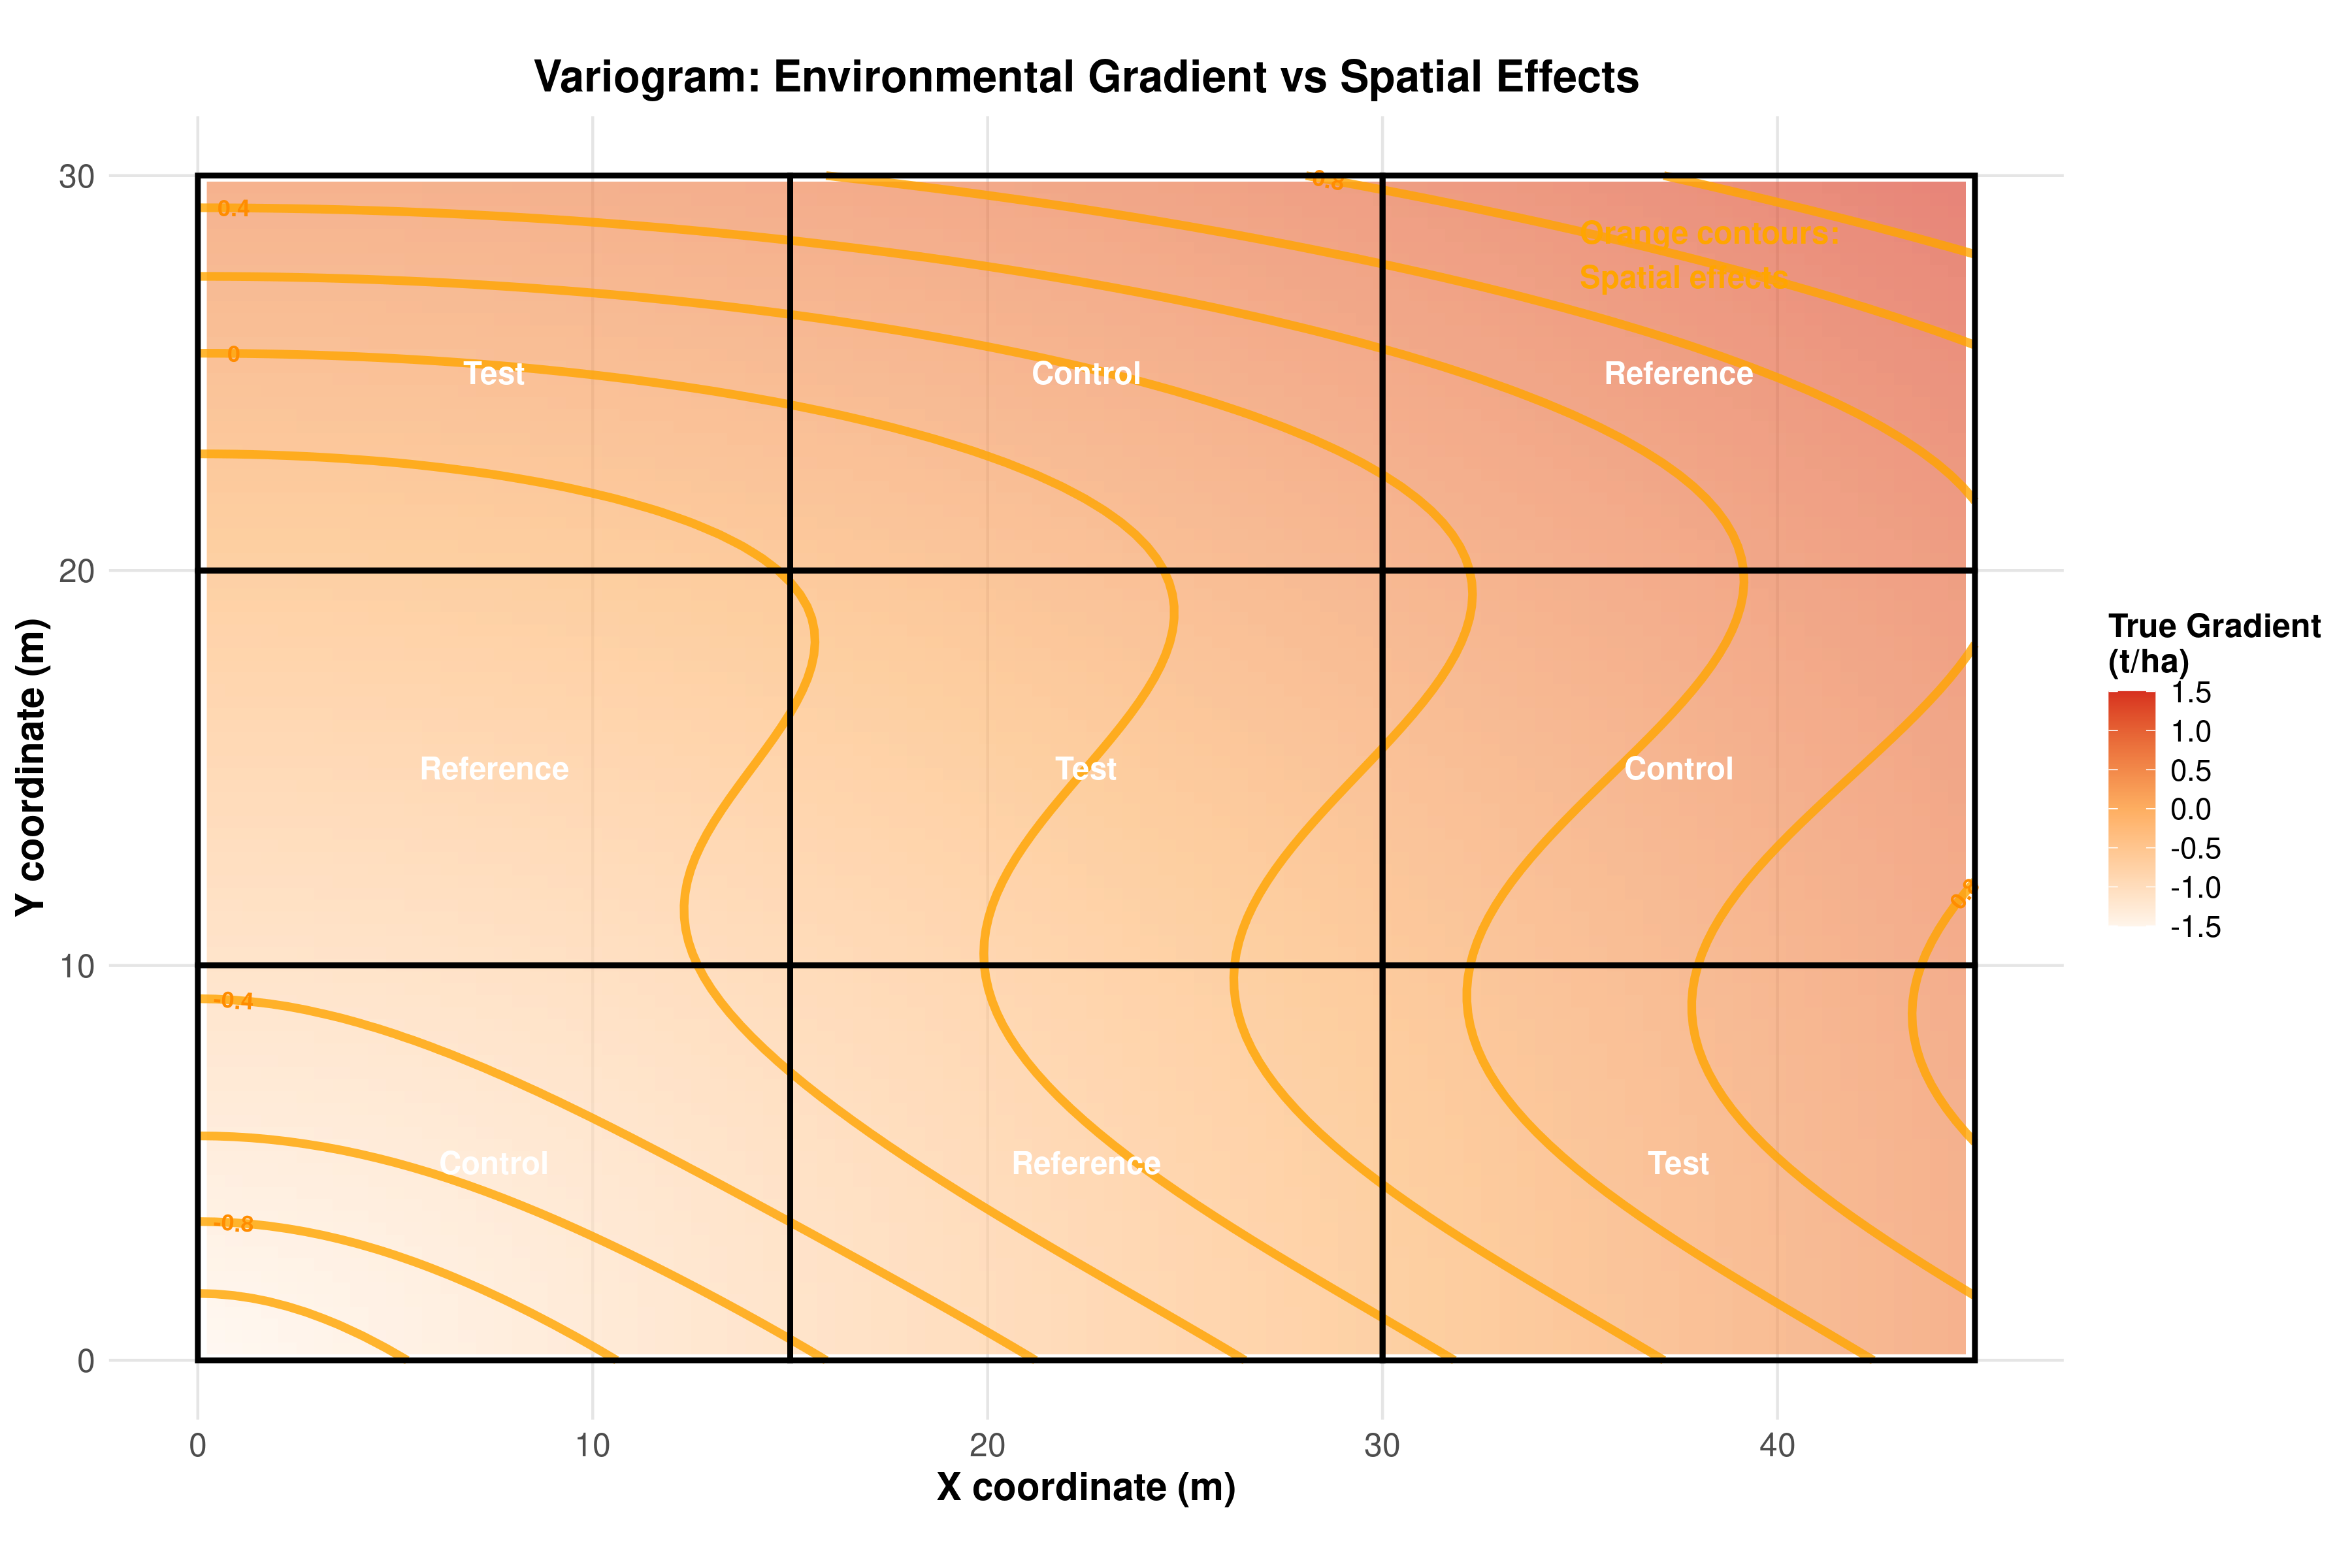
\includegraphics[width=0.95\textwidth]{Imgs/variogram_trial_design_spatial.png}
                \vspace{0.5em}
                \scriptsize
                \textcolor{blue}{Blue: True environmental gradient}
                \textcolor{orange}{Orange: Estimated spatial effect}
            \end{block}
        \end{column}
        \begin{column}{0.45\textwidth}
            \begin{block}{Model Formula}
                \vspace{0.5em}
                \begin{align*}
                    Y(s) &= \mu + X(s)\beta + Z(s) \\
                    \mu &: \text{Overall mean} \\
                    X(s)\beta &: \text{Treatment effect} \\
                    Z(s) &: \text{Spatial effect (covariance)}
                \end{align*}
            \end{block}
        \end{column}
    \end{columns}
\end{frame}

% --- SpATS Model: Trial Design and Spline Effects ---
\begin{frame}
    \frametitle{SpATS: Trial Design and Spline Effects}
    \begin{columns}[T]
        \begin{column}{0.55\textwidth}
            \begin{block}{Trial Design with Environmental Gradient}
                \centering
                % Replace with actual plot file
                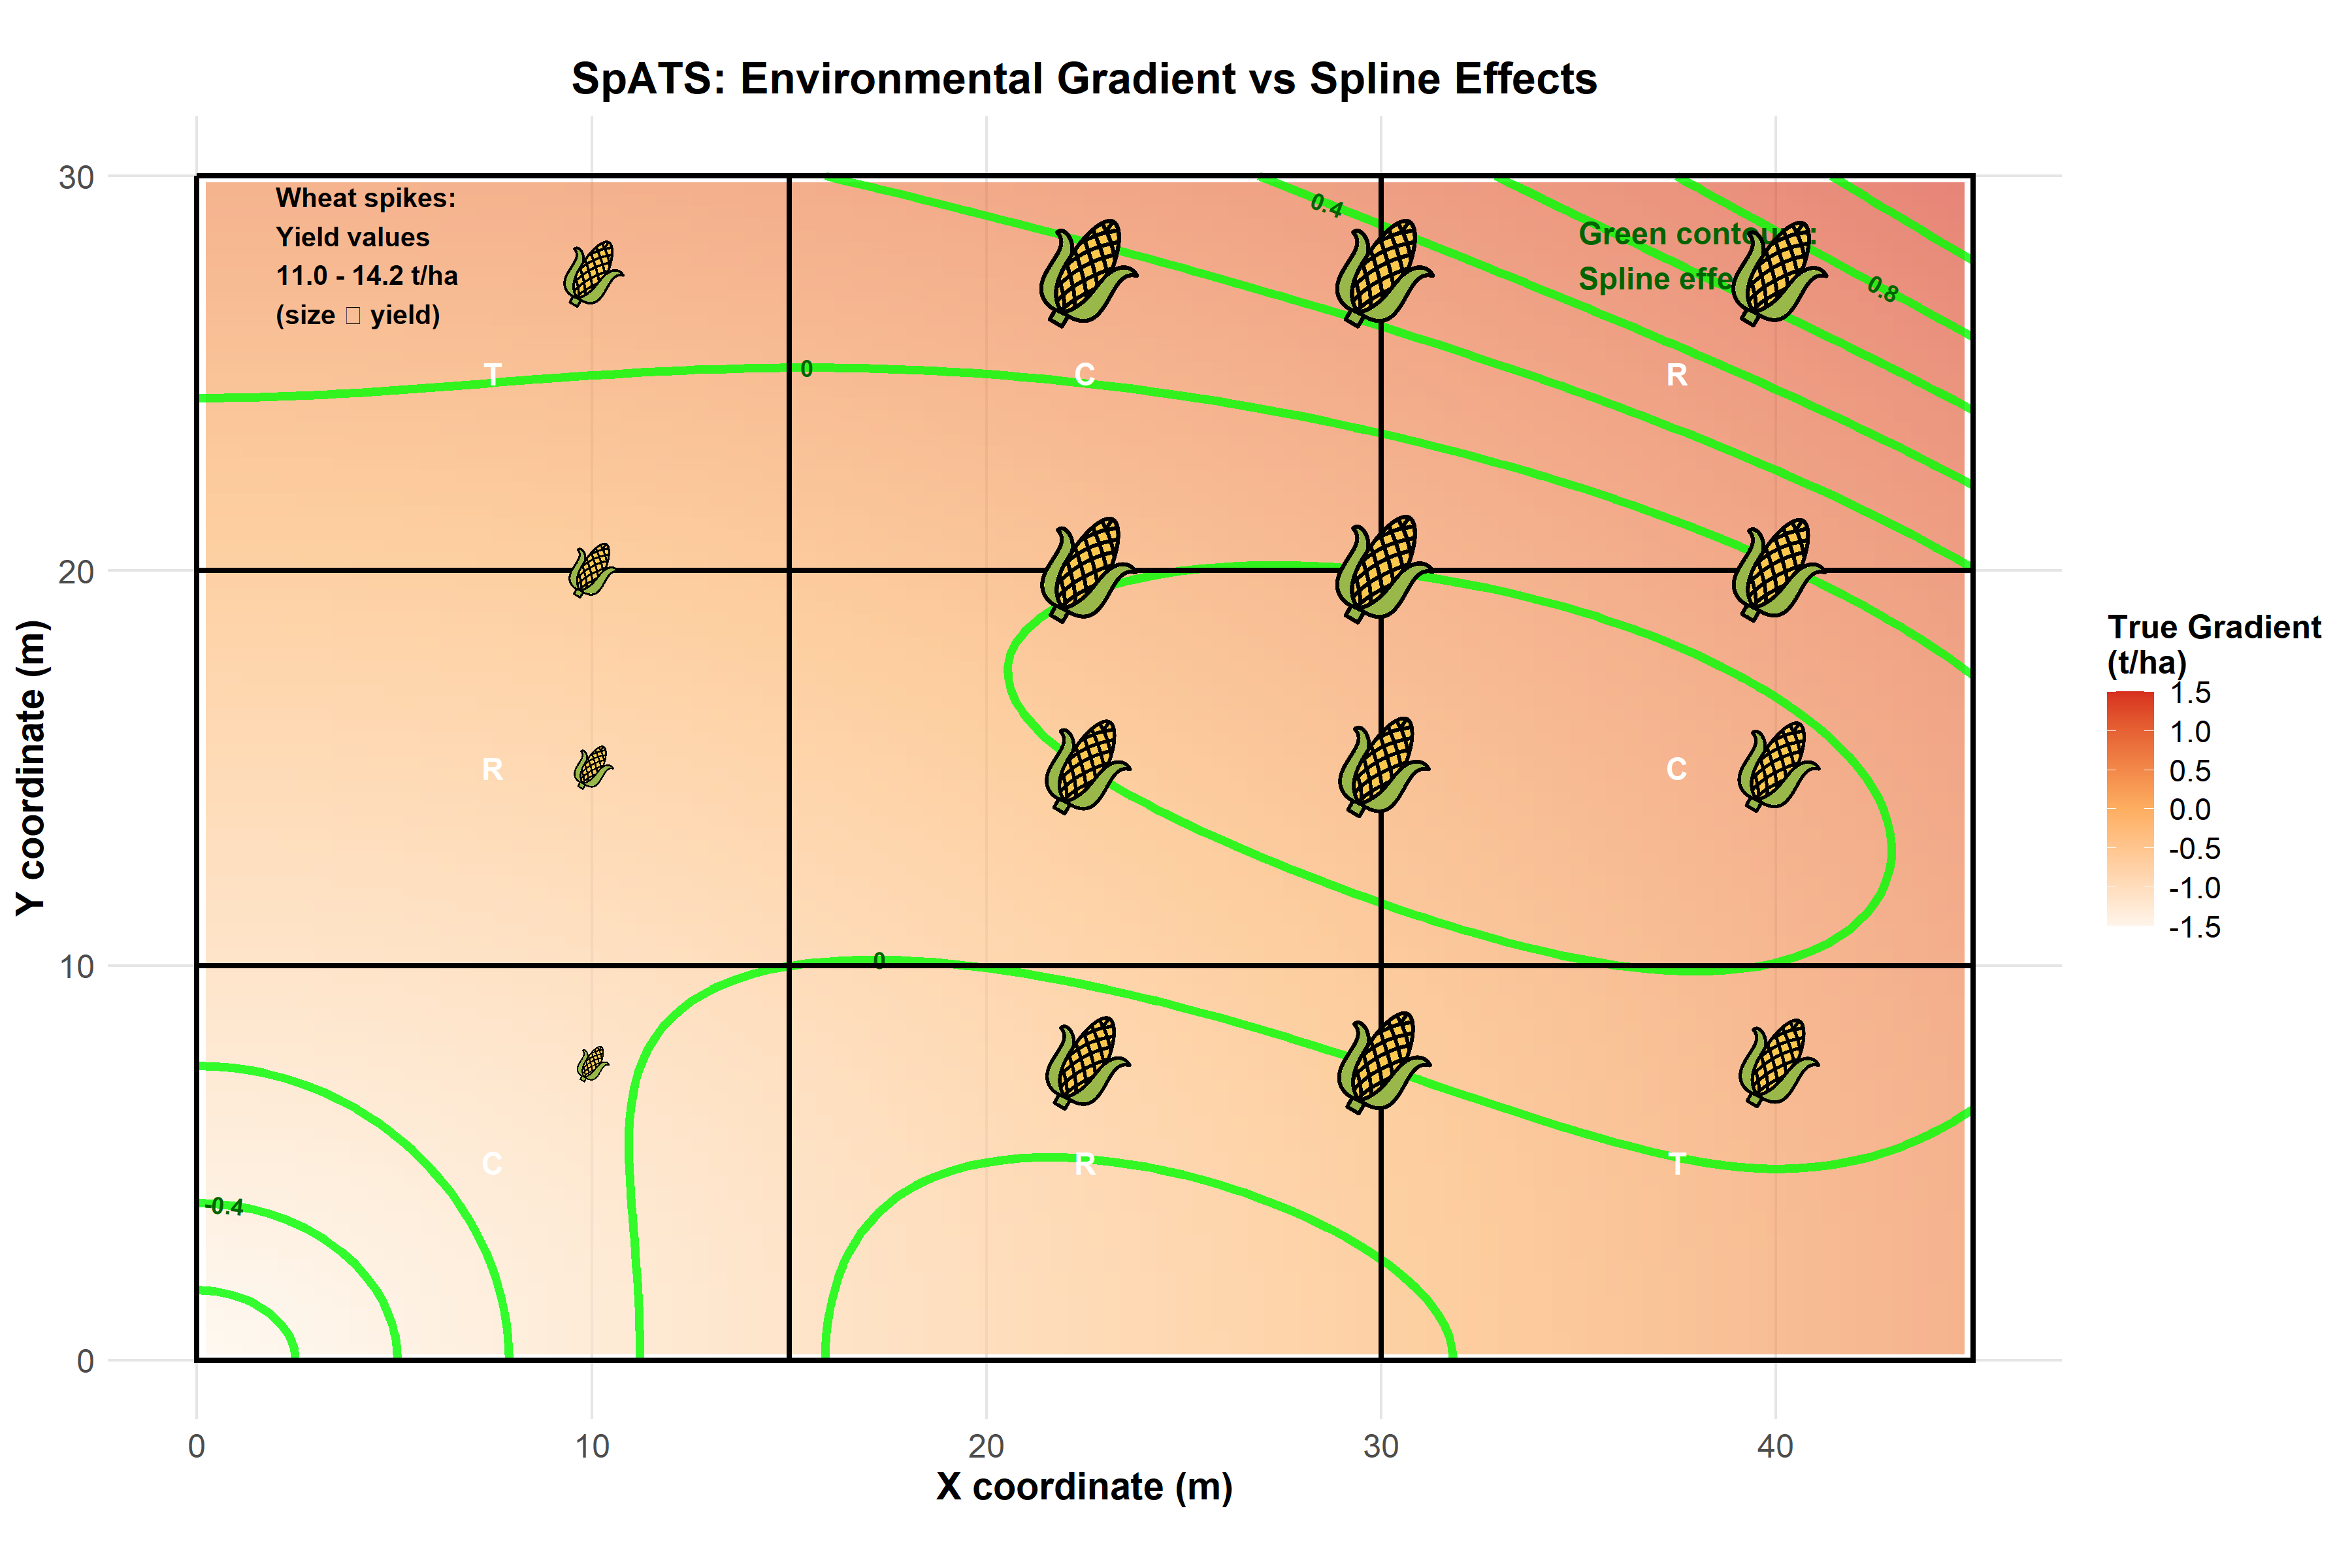
\includegraphics[width=0.95\textwidth]{Imgs/spats_trial_design_spline.png}
                \vspace{0.5em}
                \scriptsize
                \textcolor{blue}{Blue: True environmental gradient}
                \textcolor{green}{Green: Estimated spline spatial effect}
            \end{block}
        \end{column}
        \begin{column}{0.45\textwidth}
            \begin{block}{Model Formula}
                \vspace{0.5em}
                \begin{align*}
                    Y &= X\beta + f(x, y) + \varepsilon \\
                    X\beta &: \text{Treatment effect} \\
                    f(x, y) &: \text{Smooth spatial surface} \\
                    \varepsilon &: \text{Random error}
                \end{align*}
            \end{block}
        \end{column}
    \end{columns}
\end{frame}

% --- Summary Table: Estimated Effects ---
\begin{frame}
    \frametitle{Summary of Estimated Effects}
    \begin{table}[h]
        \centering
        \scriptsize
        \begin{tabular}{|l|c|c|c|c|}
            \hline
            \rowcolor{lightblue}
            \textbf{Model} & \textbf{Treatment Effect (Test)} & \textbf{Treatment Effect (Reference)} & \textbf{Environmental Effect} & \textbf{R$^2$} \\
            \hline
            \rowcolor{lightgray}
            RCBD & +2.41 & +2.03 & Block (0.47, 0.91) & 0.994 \\
            \hline
            Variogram & +2.41 & +2.03 & Spatial (Sill: 0.121, Range: 1.35m) & 0.994 \\
            \hline
            \rowcolor{lightgray}
            SpATS & +2.41 & +2.03 & Spline (6.8\% variance) & 0.994 \\
            \hline
        \end{tabular}
        \caption{Comparison of estimated effects for each model}
    \end{table}
\end{frame}

\end{document}
